
%%%%%%%%%%%%%%%%%%%%%%% file typeinst.tex %%%%%%%%%%%%%%%%%%%%%%%%%
%
% This is the LaTeX source for the instructions to authors using
% the LaTeX document class 'llncs.cls' for contributions to
% the Lecture Notes in Computer Sciences series.
% http://www.springer.com/lncs       Springer Heidelberg 2006/05/04
%
% It may be used as a template for your own input - copy it
% to a new file with a new name and use it as the basis
% for your article.
%
% NB: the document class 'llncs' has its own and detailed documentation, see
% ftp://ftp.springer.de/data/pubftp/pub/tex/latex/llncs/latex2e/llncsdoc.pdf
%
%%%%%%%%%%%%%%%%%%%%%%%%%%%%%%%%%%%%%%%%%%%%%%%%%%%%%%%%%%%%%%%%%%%


\documentclass[runningheads,a4paper]{llncs}
\usepackage{listings}
\usepackage{amssymb}
\usepackage{amsmath}
\setcounter{tocdepth}{3}
\usepackage{graphicx}
%\usepackage{comment}
\usepackage{tikz}
\usepackage{float}
%%\usepackage{subfig}
\usepackage{url}
\usepackage{todonotes}
\usepackage{float}
\usepackage{courier}

%\usepackage{subfloat}
\usepgflibrary{arrows}
\usetikzlibrary{arrows,decorations.pathmorphing,backgrounds,fit}
\usetikzlibrary{shapes.geometric}
\usepgflibrary{shapes.geometric}
\usetikzlibrary{shapes.symbols}
\usepgflibrary{shapes.callouts}
\usetikzlibrary{shapes.callouts}


\usetikzlibrary{through} 
\usepackage{tikz}
\usetikzlibrary{arrows}
\usetikzlibrary{automata}
\usetikzlibrary{backgrounds}
\usetikzlibrary{calc}
\usetikzlibrary{fit}
\usetikzlibrary{shapes}
\usetikzlibrary{snakes}


\tikzset{sortTZ/.style ={}}
\tikzset{subsortTZ/.style = {draw, <-}}
\tikzset{isomorphicTZ/.style = {subsortTZ, <->}}
\tikzset{fixedTextHeightProblem/.style = {text height=1.5ex,text depth=.25ex}}

%%%%%%%%%%%%%%%%%%%%%%%%%%%%%%%%%%%%%%%%%%%%%%%%%%%%%%%%%%%%
%                                                          %
%                                                          %
% Railway macros                                           %
%                                                          %
%                                                          %
%%%%%%%%%%%%%%%%%%%%%%%%%%%%%%%%%%%%%%%%%%%%%%%%%%%%%%%%%%%%

%%%%%%%%%%%%%%%%%%%%%%%%%%%%%%%%%%%%%%%%%%%%%%%%%%%%%%%%%%%%
%% Customiseable Lengths
%%%%%%%%%%%%%%%%%%%%%%%%%%%%%%%%%%%%%%%%%%%%%%%%%%%%%%%%%%%%

\newcommand{\RWConnectorHalfHeight}{1mm}
\newcommand{\RWPointHeight}{15mm}
\newcommand{\RWPointHalfWidth}{10mm}
%% The lengths of the units attached to the point within the junction
\newcommand{\RWJunctionUnitLength}{10mm}
%% The gap vertical between the platform edge and the track
\newcommand{\RWPlatformGapFromTrack}{2mm}
%% The gap horizontal gap between the platform edge and the connector
\newcommand{\RWPlatformGapFromConnector}{5mm}
%% The vertical height of the platform
\newcommand{\RWPlatformHeight}{3mm}

\newcommand{\RWSignalHeight}{6mm}

\newcommand{\RWSemiLongPointHalfWidth}{20mm}
\newcommand{\RWLongPointHalfWidth}{30mm}

%%%%%%%%%%%%%%%%%%%%%%%%%%%%%%%%%%%%%%%%%%%%%%%%%%%%%%%%%%%%
%% Connectors
%%%%%%%%%%%%%%%%%%%%%%%%%%%%%%%%%%%%%%%%%%%%%%%%%%%%%%%%%%%%

% param 1 = name of connector (must not exist)
% param 2 = coordinate for center of connector
\newcommand{\RWConnector}[2]{
  \coordinate (#1) at #2;
  \draw ($(#1) +(0,-\RWConnectorHalfHeight)$) -- ($(#1) +(0,+\RWConnectorHalfHeight)$);
}

% param 1 = name of connector to draw at (must exist)
% param 2 = label to be used on connector
\newcommand{\RWLabelConnectorBelow}[2]{
  \node [anchor = north] at ($(#1) +(0,-\RWConnectorHalfHeight)$) {#2};
}

% param 1 = name of connector to label (must exist)
% param 2 = label to be used on connector
\newcommand{\RWLabelConnectorAbove}[2]{
b  \node [anchor = south] at ($(#1) +(0,+\RWConnectorHalfHeight)$) {#2};
}




% param 1 = name of connector 1 (must exist)
% param 2 = name of connector 2 (must exist)
% param 3 = label to be used on linear unit
\newcommand{\RWLabelPointAboveRight}[3]{
  \node [anchor = north] at ($(#1)!.5!(#2) +(0.4,6*\RWConnectorHalfHeight)$) {#3};
}


% param 1 = name of connector 1 (must exist)
% param 2 = name of connector 2 (must exist)
% param 3 = label to be used on linear unit
\newcommand{\RWLabelPointAboveLeft}[3]{
  \node [anchor = north] at ($(#1)!.5!(#2) +(-0.4,6*\RWConnectorHalfHeight)$) {#3};
}

% param 1 = name of connector 1 (must exist)
% param 2 = name of connector 2 (must exist)
% param 3 = label to be used on linear unit
\newcommand{\RWLabelPointAbove}[3]{
  \node [anchor = north] at ($(#1)!.5!(#2) +(0,6*\RWConnectorHalfHeight)$) {#3};
}

% param 1 = name of connector 1 (must exist)
% param 2 = name of connector 2 (must exist)
% param 3 = label to be used on linear unit
\newcommand{\RWLabelLinearUnitAbove}[3]{
  \node [anchor = north] at ($(#1)!.5!(#2) +(0,5.2*\RWConnectorHalfHeight)$) {#3};
}

% param 1 = name of connector 1 (must exist)
% param 2 = name of connector 2 (must exist)
% param 3 = label to be used on linear unit
\newcommand{\RWLabelLinearUnitBelow}[3]{
  \node [anchor = north] at ($(#1)!.5!(#2) +(0,-1.2*\RWConnectorHalfHeight)$) {#3};
}

% param 1 = name of connector 1 (must exist)
% param 2 = name of connector 2 (must exist)
% param 3 = label to be used on linear unit
\newcommand{\RWLinearUnitAbove}[3] {
  \draw (#1) -- (#2);
  \RWLabelLinearUnitAbove{#1}{#2}{#3}
}
% param 1 = name of connector 1 (must exist)
% param 2 = name of connector 2 (must exist)
% param 3 = label to be used on linear unit
\newcommand{\RWLinearUnitBelow}[3] {
  \draw (#1) -- (#2);
  \RWLabelLinearUnitBelow{#1}{#2}{#3}
}

% param 1 = name of connector 1 (must exist)
% param 2 = name of connector 2 (must exist)
% param 3 = label to be used on linear unit
\newcommand{\RWOverlapAbove}[3] {
  \draw (#1) -- (#2);
 %% \coordinate (#1) at #2;
  \draw ($(#2) -(0.1,-\RWConnectorHalfHeight)$) -- ($(#2) -(0,-\RWConnectorHalfHeight)$);
  \draw ($(#2) -(0.1,+\RWConnectorHalfHeight)$) -- ($(#2) -(0,+\RWConnectorHalfHeight)$);
  \RWLabelLinearUnitAbove{#1}{#2}{#3}
}

% param 1 = name of connector 1 (must exist)
% param 2 = name of connector 2 (must exist)
% param 3 = label to be used on linear unit
\newcommand{\RWOverlapReverseAbove}[3] {
  \draw (#1) -- (#2);
 %% \coordinate (#1) at #2;
  \draw ($(#1) +(0.1,-\RWConnectorHalfHeight)$) -- ($(#1) +(0,-\RWConnectorHalfHeight)$);
  \draw ($(#1) +(0.1,+\RWConnectorHalfHeight)$) -- ($(#1) +(0,+\RWConnectorHalfHeight)$);
  \RWLabelLinearUnitAbove{#1}{#2}{#3}
}

% param 1 = name of connector 1 (must exist)
% param 2 = name of connector 2 (must exist)
% param 3 = label to be used on linear unit
\newcommand{\RWOverlapBelow}[3] {
  \draw (#1) -- (#2);
 %% \coordinate (#1) at #2; 
  \draw ($(#2) -(0.1,-\RWConnectorHalfHeight)$) -- ($(#2) -(0,-\RWConnectorHalfHeight)$);
  \draw ($(#2) -(0.1,+\RWConnectorHalfHeight)$) -- ($(#2) -(0,+\RWConnectorHalfHeight)$);
  \RWLabelLinearUnitBelow{#1}{#2}{#3}
}

\newcommand{\RWOverlapReverseBelow}[3] {
  \draw (#1) -- (#2);
 %% \coordinate (#1) at #2;
  \draw ($(#1) +(0.1,-\RWConnectorHalfHeight)$) -- ($(#1) +(0,-\RWConnectorHalfHeight)$);
  \draw ($(#1) +(0.1,+\RWConnectorHalfHeight)$) -- ($(#1) +(0,+\RWConnectorHalfHeight)$);
  \RWLabelLinearUnitBelow{#1}{#2}{#3}
}


%%%%%%%%%%%%%%%%%%%%%%%%%%%%%%%%%%%%%%%%%%%%%%%%%%%%%%%%%%%%
%% Points
%%%%%%%%%%%%%%%%%%%%%%%%%%%%%%%%%%%%%%%%%%%%%%%%%%%%%%%%%%%%

%    /----
% --------
% param 1 = name for center of point (must not exist)
% param 2 = name for center of left connector (must not exist)
% param 3 = name for center of normal connector (must not exist)
% param 4 = name for center of reverse connector (must not exist)
% param 5 = coordinate for center of point
\newcommand{\RWPoint}[5]{
  \coordinate (#1) at #5;
  \RWConnector{#2}{($#5 + (-\RWPointHalfWidth,0)$)}
  \RWConnector{#3}{($#5 + (\RWPointHalfWidth,0)$)}
  \RWConnector{#4}{($#5 + (\RWPointHalfWidth,\RWPointHeight)$)}

  \draw (#2) -- #5;
  \draw #5 -- (#3);
  \draw #5 -- (#4);
}

% --------
%    \----

% param 1 = name for center of point (must not exist)
% param 2 = name for center of left connector (must not exist)
% param 3 = name for center of normal connector (must not exist)
% param 4 = name for center of reverse connector (must not exist)
% param 5 = coordinate for center of point
\newcommand{\RWPointUpsideDown}[5]{
  \coordinate (#1) at #5;
  \RWConnector{#2}{($#5 + (-\RWPointHalfWidth,0)$)}
  \RWConnector{#3}{($#5 + (\RWPointHalfWidth,0)$)}
  \RWConnector{#4}{($#5 + (\RWPointHalfWidth,-\RWPointHeight)$)}

  \draw (#2) -- #5;
  \draw #5 -- (#3);
  \draw #5 -- (#4);
}

% ----\
% ---------
% param 1 = name for center of point (must not exist)
% param 2 = name for center of right connector (must not exist)
% param 3 = name for center of normal connector (must not exist)
% param 4 = name for center of reverse connector (must not exist)
% param 5 = coordinate for center of point
\newcommand{\RWPointReverse}[5]{
  \coordinate (#1) at #5;
  \RWConnector{#2}{($#5 + (+\RWPointHalfWidth,0)$)}
  \RWConnector{#3}{($#5 + (-\RWPointHalfWidth,0)$)}
  \RWConnector{#4}{($#5 + (-\RWPointHalfWidth,\RWPointHeight)$)}

  \draw (#2) -- #5;
  \draw #5 -- (#3);
  \draw #5 -- (#4);
}


% ---------
%     /----
% param 1 = name for center of point (must not exist)
% param 2 = name for center of right connector (must not exist)
% param 3 = name for center of normal connector (must not exist)
% param 4 = name for center of reverse connector (must not exist)
% param 5 = coordinate for center of point
\newcommand{\RWPointReverseUpsideDown}[5]{
  \coordinate (#1) at #5;
  \RWConnector{#2}{($#5 + (+\RWPointHalfWidth,0)$)}
  \RWConnector{#3}{($#5 + (-\RWPointHalfWidth,0)$)}
  \RWConnector{#4}{($#5 + (-\RWPointHalfWidth,-\RWPointHeight)$)}

  \draw (#2) -- #5;
  \draw #5 -- (#3);
  \draw #5 -- (#4);
}



%%%%%%%%%%%%%%%%%%%%%%%%%%%%%%%%%%%%%%%%%%%%%%%%%%%%%%%%%%%%
%% LongPoints
%%%%%%%%%%%%%%%%%%%%%%%%%%%%%%%%%%%%%%%%%%%%%%%%%%%%%%%%%%%%

%    /----
% --------
% param 1 = name for center of point (must not exist)
% param 2 = name for center of left connector (must not exist)
% param 3 = name for center of normal connector (must not exist)
% param 4 = name for center of reverse connector (must not exist)
% param 5 = coordinate for center of point
\newcommand{\RWLongPoint}[5]{
  \coordinate (#1) at #5;
  \RWConnector{#2}{($#5 + (-3*\RWPointHalfWidth,0)$)}
  \RWConnector{#3}{($#5 + (\RWPointHalfWidth,0)$)}
  \RWConnector{#4}{($#5 + (\RWPointHalfWidth,\RWPointHeight)$)}

  \draw (#2) -- #5;
  \draw #5 -- (#3);
  \draw #5 -- (#4);
}

% --------
%    \----

% param 1 = name for center of point (must not exist)
% param 2 = name for center of left connector (must not exist)
% param 3 = name for center of normal connector (must not exist)
% param 4 = name for center of reverse connector (must not exist)
% param 5 = coordinate for center of point
\newcommand{\RWLongPointUpsideDown}[5]{
  \coordinate (#1) at #5;
  \RWConnector{#2}{($#5 + (-3*\RWPointHalfWidth,0)$)}
  \RWConnector{#3}{($#5 + (\RWPointHalfWidth,0)$)}
  \RWConnector{#4}{($#5 + (\RWPointHalfWidth,-\RWPointHeight)$)}

  \draw (#2) -- #5;
  \draw #5 -- (#3);
  \draw #5 -- (#4);
}

% ----\
% ---------
% param 1 = name for center of point (must not exist)
% param 2 = name for center of right connector (must not exist)
% param 3 = name for center of normal connector (must not exist)
% param 4 = name for center of reverse connector (must not exist)
% param 5 = coordinate for center of point
\newcommand{\RWLongPointReverse}[5]{
  \coordinate (#1) at #5;
  \RWConnector{#2}{($#5 + (\RWLongPointHalfWidth,0)$)}
  \RWConnector{#3}{($#5 + (-\RWPointHalfWidth,0)$)}
  \RWConnector{#4}{($#5 + (-\RWPointHalfWidth,\RWPointHeight)$)}

  \draw (#2) -- #5;
  \draw #5 -- (#3);
  \draw #5 -- (#4);
}


% ----\
% ---------
% param 1 = name for center of point (must not exist)
% param 2 = name for center of right connector (must not exist)
% param 3 = name for center of normal connector (must not exist)
% param 4 = name for center of reverse connector (must not exist)
% param 5 = coordinate for center of point
\newcommand{\RWSemiLongPointReverse}[5]{
  \coordinate (#1) at #5;
  \RWConnector{#2}{($#5 + (\RWPointHalfWidth,0)$)}
  \RWConnector{#3}{($#5 + (-\RWSemiLongPointHalfWidth,0)$)}
  \RWConnector{#4}{($#5 + (-\RWPointHalfWidth,\RWPointHeight)$)}

  \draw (#2) -- #5;
  \draw #5 -- (#3);
  \draw #5 -- (#4);
}




% ---------
%     /----
% param 1 = name for center of point (must not exist)
% param 2 = name for center of right connector (must not exist)
% param 3 = name for center of normal connector (must not exist)
% param 4 = name for center of reverse connector (must not exist)
% param 5 = coordinate for center of point
\newcommand{\RWLongPointReverseUpsideDown}[5]{
  \coordinate (#1) at #5;
  \RWConnector{#2}{($#5 + (\RWPointHalfWidth,0)$)}
  \RWConnector{#3}{($#5 + (-3*\RWPointHalfWidth,0)$)}
  \RWConnector{#4}{($#5 + (-\RWPointHalfWidth,-\RWPointHeight)$)}

  \draw (#2) -- #5;
  \draw #5 -- (#3);
  \draw #5 -- (#4);
}



%%%%%%%%%%%%%%%%%%%%%%%%%%%%%%%%%%%%%%%%%%%%%%%%%%%%%%%%%%%%
%% Junctions
%%%%%%%%%%%%%%%%%%%%%%%%%%%%%%%%%%%%%%%%%%%%%%%%%%%%%%%%%%%%

%    /----
% --------
% param 1 = name for center of point (must not exist)
% param 2 = name for center of left connector (must not exist)
% param 3 = name for center of normal connector (must not exist)
% param 4 = name for center of reverse connector (must not exist)
% param 5 = coordinate for center of point
% param 6 = label for linner unit 1 - left
% param 7 = label for linner unit 2 - normal
% param 8 = label for linner unit 3 - reverse
% param 9 = label for the point
\newcommand{\RWJunction}[9]{
  %% We assume RWTempA, RWTempB and RWTempC coordinate names are not
  %% used. These can be reused as they are just overwritten.
  \RWPoint{#1}{RWTempA}{RWTempB}{RWTempC}{#5} 
  \RWConnector{#2}{($(RWTempA) + (-\RWJunctionUnitLength,0)$)}
  \RWConnector{#3}{($(RWTempB) + (+\RWJunctionUnitLength,0)$)}
  \RWConnector{#4}{($(RWTempC) + (+\RWJunctionUnitLength,0)$)}
  \draw (RWTempA) -- (#2);
  \draw (RWTempB) -- (#3);
  \draw (RWTempC) -- (#4);
  \node[anchor = north] at ($(RWTempA)!.5!(#2)$) {#6};
  \node[anchor = north] at ($(RWTempB)!.5!(#3)$) {#7};
  \node[anchor = south] at ($(RWTempC)!.5!(#4)$) {#8};
  \node[anchor = north] at ($(RWTempA)!.5!(RWTempB)$) {#9};
}

% ----\
% ---------
% param 1 = name for center of point (must not exist)
% param 2 = name for center of right connector (must not exist)
% param 3 = name for center of normal connector (must not exist)
% param 4 = name for center of reverse connector (must not exist)
% param 5 = coordinate for center of point
% param 6 = label for linner unit 1 - right
% param 7 = label for linner unit 2 - normal
% param 8 = label for linner unit 3 - reverse
% param 9 = label for the point
\newcommand{\RWJunctionReverse}[9]{
  %% We assume RWTempA, RWTempB and RWTempC coordinate names are not
  %% used. These can be reused as they are just overwritten.
  \RWPointReverse{#1}{RWTempA}{RWTempB}{RWTempC}{#5}
  \RWConnector{#2}{($(RWTempA) + (+\RWJunctionUnitLength,0)$)}
  \RWConnector{#3}{($(RWTempB) + (-\RWJunctionUnitLength,0)$)}
  \RWConnector{#4}{($(RWTempC) + (-\RWJunctionUnitLength,0)$)}
  \draw (RWTempA) -- (#2);
  \draw (RWTempB) -- (#3);
  \draw (RWTempC) -- (#4);
  \node[anchor = north] at ($(RWTempA)!.5!(#2)$) {#6};
  \node[anchor = north] at ($(RWTempB)!.5!(#3)$) {#7};
  \node[anchor = south] at ($(RWTempC)!.5!(#4)$) {#8};
  \node[anchor = north] at ($(RWTempA)!.5!(RWTempB)$) {#9};
}

%%%%%%%%%%%%%%%%%%%%%%%%%%%%%%%%%%%%%%%%%%%%%%%%%%%%%%%%%%%%
%% Platforms
%%%%%%%%%%%%%%%%%%%%%%%%%%%%%%%%%%%%%%%%%%%%%%%%%%%%%%%%%%%%

% Make a platform between two connectors assuming the connectors have
% the same y values and that the first is positioned to the left of
% the second.
% A platform also joins the connectors with a track (a line)
% param 1 = name of the platform (must not exist)
% param 2 = name of the first connector (must exist)
% param 3 = name of the second connector (must exist)
\newcommand{\RWPlatformAbove}[3]{
  \draw[fill=gray] ($(#2) + (\RWPlatformGapFromConnector,\RWPlatformGapFromTrack)$) -- ($(#3) + (-\RWPlatformGapFromConnector,\RWPlatformGapFromTrack)$) -- 
    ($(#3) + (-\RWPlatformGapFromConnector,\RWPlatformGapFromTrack) + (0,\RWPlatformHeight)$) -- ($(#2) + (\RWPlatformGapFromConnector,\RWPlatformGapFromTrack) + (0,\RWPlatformHeight)$) --
    cycle;

  \coordinate (#1) at ($(#2)!.5!(#3) + (0,\RWPlatformGapFromTrack) + 0.5*(0, \RWPlatformHeight)$);
  \draw (#2) -- (#3);
}

% Make a platform between two connectors assuming the connectors have
% the same y values and that the first is positioned to the left of
% the second.
% A platform also joins the connectors with a track (a line)
% param 1 = name of the platform (must not exist)
% param 2 = name of the first connector (must exist)
% param 3 = name of the second connector (must exist)
\newcommand{\RWPlatformBelow}[3]{
  \draw[fill=gray] ($(#2) + (\RWPlatformGapFromConnector,-\RWPlatformGapFromTrack)$) -- ($(#3) + (-\RWPlatformGapFromConnector,-\RWPlatformGapFromTrack)$) -- 
    ($(#3) + (-\RWPlatformGapFromConnector,-\RWPlatformGapFromTrack) + (0,-\RWPlatformHeight)$) -- ($(#2) + (\RWPlatformGapFromConnector,-\RWPlatformGapFromTrack) + (0,-\RWPlatformHeight)$) --
    cycle;

  \coordinate (#1) at ($(#2)!.5!(#3) + (0,-\RWPlatformGapFromTrack) + 0.5*(0, -\RWPlatformHeight)$);
  \draw (#2) -- (#3);
}

% param 1 = name of the platform to label (must exist)
% param 2 = label to be used on platform
\newcommand{\RWLabelPlatformAbove}[2]{
  \node [anchor = south] at ($(#1) + 0.5*(0, \RWPlatformHeight)$) {#2};
}

% param 1 = name of the platform to label (must exist)
% param 2 = label to be used on platform
\newcommand{\RWLabelPlatformBelow}[2]{
  \node [anchor = north] at ($(#1) + 0.5*(0, -\RWPlatformHeight)$) {#2};
}



\newcommand{\RWTrainAbove}[3]{
  \draw[fill=gray] ($(#2) + (2.5*\RWPlatformGapFromConnector,1.2*\RWPlatformGapFromTrack)$) -- ($(#3) + (-2.5*+\RWPlatformGapFromConnector,1.2*\RWPlatformGapFromTrack)$) -- 
    ($(#3) + (-2.7*\RWPlatformGapFromConnector,1.2*\RWPlatformGapFromTrack) + (0,\RWPlatformHeight)$) -- ($(#2) + (2.7*\RWPlatformGapFromConnector,1.2*\RWPlatformGapFromTrack) + (0,\RWPlatformHeight)$) --
    cycle;

  \coordinate (#1) at ($(#2)!.5!(#3) + (0,\RWPlatformGapFromTrack) + 0.5*(0, \RWPlatformHeight)$);
  \draw (#2) -- (#3);
}


% param 1 = name of connector (must not exist)
% param 2 = coordinate for center of connector
\newcommand{\RWSignal}[3]{
  \coordinate (#1) at #2;
  \draw ($(#1) + (-0.3,0)$) -- ($(#1) +(-0.3,+\RWSignalHeight)$); 
  
  \node[draw, inner sep=0pt, minimum size= 7pt] (A) at ($(#1) +(0,+\RWSignalHeight)$) {};

  \draw  ($(#1) +(-0.3,+\RWSignalHeight)$) -- (A.west);
  \node at ($(#1) +(0.6,+\RWSignalHeight)$)  {#3};
}

\newcommand{\RWReverseSignal}[3]{
  \coordinate (#1) at #2;
  \draw ($(#1) + (0.3,0)$) -- ($(#1) +(0.3,+\RWSignalHeight)$); 
  
  \node[circle, draw, inner sep=0pt, minimum size= 7pt] (A) at ($(#1) +(0,+\RWSignalHeight)$) {};
  \node at  ($(#1) +(0,1.7*\RWSignalHeight)$) {#3};
  \draw  (A.east) --  ($(#1) +(0.3,+\RWSignalHeight)$);
}

 
\lstset{basicstyle=\fontsize{8}{8}\ttfamily, xleftmargin=2em, framexleftmargin=1.5em, framexrightmargin=-0.6em, frame=single}

\begin{document}
\mainmatter 

\title{Towards Safety Analysis of ERTMS/ETCS \\ Level 2 in Real-Time
  Maude}

\titlerunning{ERTMS/ETCS Level 2 in Real-Time Maude}

\author{Phillip James\inst{1} \and Andrew Lawrence \inst{2} \and \\ 
Markus Roggenbach\inst{1} \and  Monika Seisenberger\inst{1}}
%
\institute{Swansea University, UK
\and
Hitachi Data Systems, Poole, UK.
}

\authorrunning{James, Lawrence, Roggenbach, Seisenberger}

\maketitle

\begin{abstract}
ERTMS/ETCS is a European signalling, control and train protection
system. In this paper, we model and analyse this complex system of
systems, including its hybrid elements, on the design level in
Real-Time Maude. Our modelling allows us to formulate safety
properties in physical rather than in logical terms. %% For instance ``no
%% collision between trains'' is expressed as the physical invariant: the
%% distance (in meters) between trains never falls below a minimum
%% threshold.
We systematically validate our model by simulation and error
injection. Using the Real-Time Maude model-checker, we effectively
verify a number of small rail systems.
\end{abstract}

\section{Introduction}

% “Introduction: in general, could you introduce the problem in a
% sentence or two for the non-expert? What is an interlocking”


The European Rail Traffic Management System (ERTMS) / European Train
Control System (ETCS) is a European signalling, control and train
protection system designed to allow for high speed travel, to increase
capacity, and to facilitate cross-border traffic movements
\cite{ERTMS}. ERTMS/ETCS is a complex system of systems, made up by
distributed components. It is specified at four different levels,
where each level defines a different use as a train control system. In
our paper we consider ERTMS/ETCS Level 2, which is characterised by
continuous communications between trains and a radio block centre.

The switch from classical railway signalling systems to ERTMS/ETCS
train control poses a number research questions for the formal methods
community. Can safety be guaranteed? Can formal methods be used to
confirm that such a switch improves capacity? Is it possible to
predict capacity using formal methods? To address such questions it is
necessary to develop and analyse timed or hybrid models. ERTMS/ETCS
Level 2 takes speed and braking curves of each individual train into
account. These determine the train's breaking point well in advance of
the end of authority that the signalling system had granted to this
train. Such an approach is in contrast to classical signalling
systems, which treat all trains in the same way. Therefore, they need
to be designed for worst braking. Consequently, in
formal safety analysis, such traditional systems can be treated on a purely
logical level, ignoring the aspect of time -- see, e.g.,
\cite{sttt14,JamesMNRST14}.

An ERTMS/ETCS system consists of a controller, an interlocking (a
specialised computer that determines if a request from the controller
is "safe"), a radio block centre, track equipment, and a number of
trains. While the {ERTMS/}{ETCS} standard details the interactions between
trains and track equipment (e.g., in order to obtain concise train
position information) and radio block centre and trains (e.g., to hand
out movement authorities), the details of how controller, interlocking
and radio block centre interact with each other are left to the
suppliers of signalling solutions such as our industrial partner
Siemens Rail Automation UK. In this paper we work with
the implementation as realised by Siemens. In the following we refer
to this system simply as ERTMS.

One development step when building an ERTMS system consists of
developing a so-called detailed design. Given geographical data such
as a specific track layout and what routes through this track layout
shall be used, the detailed design adds a number of tables that
determine the location specific behaviour of interlocking and radio
block centre. The objective of our modelling is to provide a formal
argument that a given detailed design is safe. Here we focus on
collision freedom, though our model is extensible to deal with 
further safety properties, and possibly also with performance
analysis.

We base our modelling approach on Real-Time Maude, which is a language
and tool supporting the formal object-oriented specification and
analysis of real-time and hybrid systems. To the best of our
knowledge, this is the fist time Maude or Real-Time Maude has been
used in the train domain. In order to obtain a faithful model of
ERTMS/ETCS level 2 on the design level, we follow a systematic
approach, established by the Swansea Railway Verification
Group.
%% %
%% First, we develop a domain specific language that allows us to
%% represent the rail yard under discussion.
%% %
%% Then, we systematically identify the system's entities and determine the
%% information flow between them.
%% %
%% Finally, we provide a number of translation tables: static elements
%% such as the track plan and the various tables are specified as data
%% types using Maude equations; the ERTMS/ETCS components are represented
%% as objects; their message exchange according to the rules laid down
%% in the standard or by Siemens is captured by rewrite rules.

This paper extends our location-specific modelling presented in
\cite{old} to a generic and far more detailed modelling. It is
organised as follows. First, we introduce the ERTMS Level 2 standard,
%describe the detailed design of a pass-through station, 
and briefly discuss high level safety properties for ERTMS. Then, we
give a short presentation of Real-Time Maude with a focus on standard
specification techniques for hybrid systems. In Section 4, we present
our modelling of ERTMS in Real-Time Maude, discussing each component
in detail. In Section 5, we validate our model by simulation and
error injection. Finally, we present model checking results and put
our approach in the context of related work.


%% Markus

\section{ERTMS Level 2}

 %% The European Rail Traffic Management System (ERTMS) consists of
 %% several sub-systems. With regards to control and safety, these
 %% systems are typically designed to ensure safe operation of a
 %% particular area of railway known as a scheme plan. The ERTMS standard
 %% also outlines mechanisms allowing trains to pass between such regions
 %% (so-called handover protocols). In our work, we concentrate on safety
 %% within one region, and leave the handover mechanism for future work.

ERTMS Level 2 extends classical railway signalling. To this end its
location specific design\footnote{We focus here on one ERTMS/ETCS
  system controlling a single, geographic region.} extends the
classical notion of a scheme plan by information used for the radio
block centre (RBC). ERTMS safety analysis also requires train
characteristics such as maximum speed, acceleration and braking
curves.

\subsection{Scheme Plans}

A scheme plan is a well-established concept within the railway
domain. Figure~\ref{fig:station} depicts such a \emph{scheme plan} for
a pass-through station. It comprises of a track plan, a control table,
release tables and RBC tables. The \emph{track plan} provides the
topological information for the station. It consists of 8 tracks
(e.g.,\ BC) each with a length, 3 marker boards (e.g.,\ MB1), and two
points (e.g.,\ P2). A topological \emph{route} is a piece of railway
on which a train can travel, (typically) between two marker boards
(e.g., from MB1 to MB2). The {\em control table} describes under which
conditions a \emph{route} can be set.\footnote{It is a design
  decision whether a topological route appears in the control table. The
  routes in the table are those available for use by trains.}  For
example, a train can only proceed on route 1A when point P1 is in
normal (straight) position and tracks AA, AB and AC are clear, i.e.,
currently not occupied by any train. The \emph{release table} is used
to implement sequential release, a technique to improve
capacity. The release table describes when a point is again free to move
after being locked for a particular route. For example, when sending a
train on route 1A, point P1 is free to move already, when this train
has reached track AC. This allows to send another train on route 1B
before the first train has reached track AD and thus completely left
route 1A. Finally, the \emph{RBC tables} are used for %movement
calculations within the RBC.

\begin{figure}[H]
  \centering
 
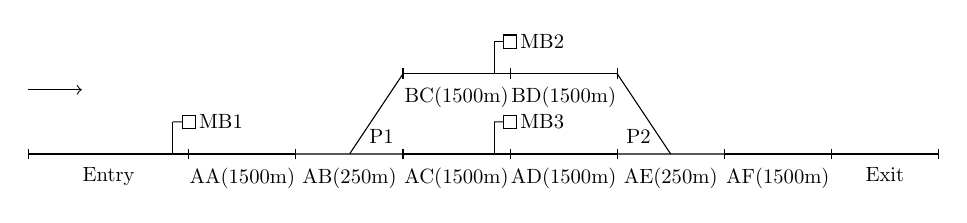
\begin{tikzpicture}[scale=0.68,transform shape]
\fontfamily{Heletvica Narrow}{\fontsize{11}{11}\selectfont
\draw [->] (0,-0.8) to (1,-0.8);

\RWConnector{a0}{(0,-2)}
\RWConnector{a1}{(3,-2)}
\RWLinearUnitBelow{a0}{a1}{Entry}
\RWSignal{MB1}{(3,-2)}{MB1}
\RWConnector{a2}{(5,-2)}
\RWLinearUnitBelow{a1}{a2}{AA(1500m)}
\RWPoint{p101}{a3}{a4}{p101}{(6,-2)}
\RWLabelPointAboveLeft{a4}{a4}{P1}
\RWLabelLinearUnitBelow{a3}{a4}{AB(250m)}

\RWConnector{b5}{(9,-0.5)}
\RWLinearUnitBelow{p101}{b5}{BC(1500m)}
\RWConnector{b6}{(11,-0.5)}
\RWLinearUnitBelow{b5}{b6}{BD(1500m)}

\RWSignal{MB2}{(9,-0.5)}{MB2}
\RWConnector{a5}{(9,-2)}
\RWLinearUnitBelow{a4}{a5}{AC(1500m)}
\RWSignal{MB3}{(9,-2)}{MB3}
\RWConnector{a6}{(11,-2)}
\RWLinearUnitBelow{a5}{a6}{AD(1500m)}

\RWPointReverse{p102}{a7}{a8}{p101}{(12,-2)}
\RWLabelPointAboveRight{a8}{a8}{P2}
\RWLabelLinearUnitBelow{a7}{a8}{AE(250m)}

%\RWSignal{MB4}{(15,-2)}{MB1}
\RWConnector{a9}{(15,-2)}
\RWLinearUnitBelow{a7}{a9}{AF(1500m)}
\RWConnector{a10}{(17,-2)}
\RWLinearUnitBelow{a9}{a10}{Exit}
}
\end{tikzpicture}
\vspace{0.5cm}

\begin{tiny}
  \begin{tabular}{lll}
  Interlocking Tables: &
\begin{tabular}{|c|c|c|c|}
\hline
Route & Clear Tracks & Normal & Reverse \\
\hline \hline
1A & AA, AB, AC & P1 & \\
1B & AA, AB, BC & & P1 \\
2  & BD, AE, AF & & P2 \\  
3  & AD, AE, AF & P2 & \\
\hline
\end{tabular}
&
\begin{tabular}{|c|c|c|}
\hline
Point & Route & Release \\
\hline \hline
P1 & 1A & AC \\
P1 & 1B & BC \\
P2 & 2 & AF \\
P2 & 3 & AF \\
\hline
\end{tabular}\\ \quad \\
RBC Tables: &
\begin{tabular}{|c|c|}
\hline
Current Position & Continuation Routes \\
\hline \hline
Before MB1 & 1A, 1B \\
Before MB2 & 2 \\
Before MB3 & 3 \\
\hline
\end{tabular}
&
\begin{tabular}{|c|c|}
\hline
Granted Route & EOA \\
\hline \hline
1A & 3249m \\
1B & 3249m \\
2 & 6499m \\
3 & 6499m \\
\hline
\end{tabular}
\end{tabular}
\end{tiny}
\caption{Scheme Plan for a pass-through station.}
\label{fig:station}\label{fig:rbctables}
\end{figure}

We consider open scheme plans with entry and exit tracks
only. Furthermore, we assume that marker boards are placed at the end
of tracks, and that the speed limit is the same for all tracks.

\subsection{ERTMS System Architecture}

Once a scheme plan has been designed, a number of control systems are
implemented based around it. In the following we %systematically
identify the entities of ERTMS, describe their abstract behaviour and
determine the abstract information flow between them in line with the
design by Siemens Rail UK, see Figure~\ref{fig:arch}.

The \emph{controller} (manual or computerised) is responsible for
controlling the flow of trains through the railway network. The
controller completes this task by sending ``route request'' messages
to the interlocking. These route requests are dependent upon elements
such as the current timetable to be adhered to and details on
congestion within the network. For simplicity, we abstract from
``route cancel'' and ``acknowledgement'' messages.

The \emph{interlocking} is responsible for setting and granting
requested routes. Once the controller has requested a route, the
interlocking will use information on current track occupation and
point settings (from the track equipment) to determine if it is safe
for the requested route to be set. Whether a route can be set or not
is computed in a process based upon the conditions stipulated by the
control table, see Figure~\ref{fig:station}. Once the interlocking has
checked that all points on the route are free to move or already in
the right position, it will send a ``route available'' message to the
RBC (Radio Block Centre). This informs the RBC that the route is free
for use, however it is not yet reserved for a train. The RBC initiates
the process of locking a route for a particular train by sending a
``request to proceed'' message to the interlocking. On receiving this
message, the interlocking will then ensure that, based on the control
table, all tracks for the route are free and that the points are
indeed locked in the required positions. Once this step is completed,
the interlocking sends a ``proceed'' message to the RBC indicating
that a train can use the route.

The \emph{RBC}'s main responsibility is to take the route information
presented by the interlocking and use it to manage the movement of
trains across geographic positions on the railway. To do this, the RBC
and trains use the notion of a \emph{movement authority}. A movement
authority is an area of geographical railway that a train is permitted
to move within. The furthest point along the railway to which a train
is permitted to move is indicated by a point known as the \emph{end of
  authority} (EoA) which is given to a train by the RBC. As a train
moves across the railway network, it uses beacons on the track to
continually calculate its position. When it is nearing its EoA, it
makes a new ``movement authority request'' to the RBC indicating that
it would like its movement authority to be extended. After receiving
this request, the RBC will map the physical location of the train to
an available continuation route that has been presented to it by the
interlocking.\footnote{At this point, there should be maximally one
  route available that matches a particular train. This is ensured by
  the requests from the controller and also the ability of the
  interlocking to deny requests for conflicting routes} This
calculation is performed based on a look-up table designed as part of
the RBC for a scheme plan, an example of such a table is provided in
Figure~\ref{fig:rbctables}. It will then issue a ``request to
proceed'' message to the interlocking for this route. Once the RBC has
received a ``proceed'' message from the interlocking, it will compute,
based on the route that has been granted, a new EoA for the
train. Again, this information is provided by a look-up table, see
Figure~\ref{fig:rbctables}. This new EoA is then finally sent as a
``movement authority'' message to the train.

With regards to \emph{trains}, their behaviour is parameterised by
maximum speed, acceleration and braking curves. We make a maximum
progress assumption for trains, i.e., trains are running as fast and
as far as possible. Namely, if a train has a movement authority beyond
its current position it will accelerate towards its maximum
speed. When the maximum speed is reached, the train will continue to
travel at this speed. Whilst accelerating or travelling at maximum
speed the train will start braking at the last possible time in order
not to overrun its EoA. Trains are guided by the track layout,
respecting the positions to which the interlocking has set points. As
trains move along the track, track equipment senses track occupation
and reports it to the interlocking.
%
%% \begin{figure}[h]
%% \centering
%% \begin{tiny}
%% \begin{tabular}{|c|c|}
%% \hline
%% Current Position & Possible Continuation Routes \\
%% \hline \hline
%% Before MB1 & 1A, 1B \\
%% Before MB2 & 2 \\
%% Before MB3 & 3 \\
%% \hline
%% \end{tabular}
%% \quad
%% \begin{tabular}{|c|c|}
%% \hline
%% Granted Route & EOA \\
%% \hline \hline
%% 1A & 3249m \\
%% 1B & 3249m \\
%% 2 & 6499m \\
%% 3 & 6499m \\
%% \hline
%% \end{tabular}
%% \end{tiny}
%% \caption{RBC tables for calculating continuation routes and end of authorities.}
%% \label{fig:rbctables}
%% \end{figure}
%
We assume that \emph{track equipment} (points, track circuits, beacons
etc.) functions correctly and that points move instantaneously. This
is justified as our verification aim is to establish correctness of
the location and train specific design parameters for a ERTMS system
for a single geographic region. Therefore, we refrain from modelling
track equipment.

\begin{figure}[H]
\centering
\includegraphics[scale=0.45]{images/Architecture.png}
\caption{ERTMS control architecture.}
\label{fig:arch}
\end{figure}

\subsection{Safety Conditions}
\label{sec:safetycond}
In the context of ERTMS, several high level safety conditions have
been discussed such as collision freedom or derailment on a point.  In
this paper, we focus on collision freedom, i.e., excluding the
possibility that two trains collide.  In the context of classical
signalling systems, this property usually is formulated logically,
e.g., we verify that there are never two trains on the same track
\cite{sttt14}. In contrast, for ERTMS we rather consider the physical
invariant: the distance between trains never falls below a
minimum threshold.

%% MR: excellent text - but we should use it in the introduction of 
%% the error-injection section
%%
%% As we illustrate later in Section\ref{sec:errorInjection}, there are a
%% number of ways in which this condition can be violated within
%% ERTMS. In this work, we assume that the generic dynamic behaviour of
%% the interlocking, RBC and any trains is correct and that the mistakes
%% we are looking for are within the parameters to these models. For
%% example, mistakes in the design of the control and release tables for
%% an interlocking can lead to a violation of this property. Similarly,
%% mistakes in the design of mappings between routes and end of
%% authorities for use within the RBC can also violate this
%% property. Finally, if a train has incorrect parameters input for
%% computing braking distances, the the property may once again be
%% violated.


%% Phil

\section{Maude/Real-Time Maude}

The Maude system \cite{MC03} is a multi-purpose tool with support for
executable specification, simulation and verification.
%
%%and our approach uses all of these capabilities.
%
Its wide range of capabilities made us to favour Maude. Particularly,
we are interested in the Maude LTL Model Checker \cite{ES00}.  Real
Time Maude \cite{PO07b} is an extension of Maude containing specific
support enabling the modelling and verification of
%
%of discrete time and 
%
real-time systems.
%
%The Real-Time Maude system contains models of discrete time based on the natural numbers and dense time based on the rational numbers.
%
%% Maude specifications are built from \emph{functional modules} 
%% %
%% %declared using \texttt{fmod} and \texttt{endfm}
%% %
%% which contain the following:
%% %
%% \begin{center}
%% \begin{tabular}{| c | l |}
%% \hline sorts & \texttt{sort} $s$ or \texttt{sorts} $s \ s' .$
%% \\ \hline subsorts & \texttt{subsort} $s < s' \ .$ \\ \hline function
%% symbols & \texttt{op} $f \ : \ s_1 \ldots s_n$ \texttt{->} $s \ .$
%% \\ \hline variables & \texttt{vars} $v \ v' : s' .$\\ \hline
%% unconditional equations &\texttt{eq} $t = t' .$\\ \hline conditional
%% equations & \texttt{ceq} $t = t'$ \texttt{if} $cond$ \\ \hline
%% membership axioms & \texttt{mb} $t \ : \ s \ .$ or \texttt{cmb} $t \ :
%% \ s$ \texttt{if} $cond \ .$ \\ \hline unconditional rules &
%% \texttt{rl} [label] : $t => t' .$ \\ \hline conditional rules &
%% \texttt{crl} [label] : $t => t'$ \texttt{if} $cond$ \\ \hline
%% \end{tabular}
%% \end{center}

Object-based systems can be modelled as multisets of objects and
messages where the messages define the communication between the
objects and typically trigger actions of the objects. A class $C$ with
attributes of \verb|a_1| to \verb|a_n| of sort \verb|Sort_1| to \verb|Sort_n|, and an object {\tt O}
with attribute values \verb|v_1| to \verb|v_n| of class {\tt C} are written as, respectively
%
\begin{lstlisting}[columns=fixed]
class C | a_1 : Sort_1, ... , a_n : Sort_n .  
< O : C | a_1 : v_1, ... , a_n : v_n > .
\end{lstlisting}
%
Objects declared together with messages
\begin{lstlisting}[columns=fixed]
msgs M_1 ... M_k : Sort_1 ... Sort_n -> Msg .  
\end{lstlisting}
form a multiset of the sort \texttt{Configuration}, a subsort of Maude's built-in sort
\texttt{System},  using \verb|__| for multiset union.
\begin{lstlisting}[columns=fixed]
sorts Object Msg Configuration .
subsort Object Msg < Configuration . 
op __ : Configuration Configuration -> Configuration [ctor] .
\end{lstlisting}

A real-time specification \cite{PO07b} consists of a sort \verb|Time|
(in our case \verb|PosRat|), the constructor
%
\verb| {_} : System -> Globalsystem|
%
with the meaning that \verb|{t}| represents the whole system (and does not appear
as an argument to another function - as is marked by using the independent type \texttt{Globalsystem}),
instantaneous rewrite rules, and a so-called tick rule that defines how time elapses.
%
As \cite{PO07}, we use the operators \verb|delta| and \verb|mte| in
order to define the effect of time elapse on a configuration, and of the
maximal possible time elapse, resp.
%
\begin{lstlisting}[columns=fixed]
op delta : Configuration Time -> Configuration [frozen (1)] . 
op mte : Configuration -> TimeInf [frozen (1)] .
\end{lstlisting}
Here, \texttt{TimeInf} is the sort \texttt{Time} enriched with an infinity element
\texttt{Inf}. These two functions are distributed
over objects and messages, i.e., each
object has the same time available, and as the maximal time elapse
for a message has value 0, time can only progress once all messages
are consumed.
%
\begin{lstlisting}[columns=fixed]
vars CON1 CON2 : NeConfiguration . var R : Time .
eq delta(none, R) = none .
eq delta(CON1 CON2, R) = delta(CON1,R) delta(CON2,R) . 
eq mte(none) = INF .
eq mte(CON1 CON2) = min(mte(CON1),mte(CON2)) .
\end{lstlisting}
%
The argument {\tt R} of type {\tt Time} is determined by the tick rule 
%
\begin{lstlisting}
crl [tick] : {CURRENT} => {delta(CURRENT,R)} in time R 
                if R <= mte(CURRENT) [nonexec] .
\end{lstlisting}
%
The default tick time is defined by
\begin{lstlisting}[columns=fixed]
(set tick def 1 .) 
\end{lstlisting}
%
This means we look at the configuration either at each time step, or
more often in the case that some event occurs, for a justification see
e.g.\ \cite{PO06}.


%% For a theoretical justification of this approach as well as completeness results see  e.g. \cite{PO06}.
%%Meseguer and O show in [completenesspaper] under which conditions
%%the specification is time robust and therefore complete.
%% In the next section we will give additional domain specific equations
%% for \verb|delta| and \verb|mte| which define the behaviour of all
%% objects involved.

%%% Andy -- Include time/mte/delta
%%% Uli has subsection on completeness.

\section{Modelling ERTMS in Maude}

To the best of our knowledge, our modelling of ERTMS is the first one
comprising all ERTMS subsystems required for the control cycle in
ERTMS/ETCS Application Level 2, c.f.\ Figure 6 in the ERTMS/ETCS
System Requirements Specification \cite{spec}. For simplicity, we
consider only uni-directional rail yards, as these exhibit many of the
components of bi-directional rail yards, but are of a lower complexity
with regards to the number of routes required within the model. Also,
we make the standard assumption that trains have no length. This is
the typical abstraction when one deals with trains whose length is
shorter than any track length in the given scheme plan. For a detailed
discussion of the topic see, e.g., our publication discussing train
length \cite{JamesMNRST14}.

In the following, we provide an overview of our model%
\footnote{The models are available at:\\
{\tt \footnotesize
 http://www.cs.swan.ac.uk/\%7Ecsmarkus/ProcessesAndData/Models}}: first we discuss the static
data types; then we look at the instantaneously reacting
sub-systems, i.e., controller, interlocking, and RBC; next, we
describe how we capture  train behaviour, which requires
differential equations describing motion; finally, we address how to
express collision-freedom. We note that our model is generic, with only
location specific data as a parameter. This location specific data has been encoded manually, however this process could be automated within OnTrack~\cite{james14c}.

%% {\sl For the purpose of reviewing, our models are available at
%% \begin{center}
%% \url{http://www.cs.swan.ac.uk/%7Ecsmarkus/Station.zip}.
%% \end{center}
%% The \%7E stands for $\sim$ -- in case the link is not clickable. In
%% case of acceptance, we will make our code available to the scientific
%% community via a stable webpage.}

\subsection{Datatypes: Location Specific Data and Messages}
%%%Topology and control/rbc tables.
%Utilising our domain specific language, see, e.g., \cite{james14}, 
We model the rail topology as a connected collection of tracks,
points, and routes and provide a systematic translation into
Maude. For the example given in Figure~\ref{fig:station}, the location
specific data Maude is encoded as follows:
%
\begin{lstlisting}[columns=fixed]
sort RouteName . ops RouteName1A ... : -> RouteName .
sort Track .     ops AA AB AC ... : -> Track        .
sort Point .     ops P1 P2 : -> Point               . 
\end{lstlisting}
%
The connection between tracks is given by a \verb|next| function. If
the track under discussion is a point, as, e.g., track \verb|AB|, it
has two potential successors, namely \verb|AC| and
\verb|BC|, depending on the current setting of the point.
%
\begin{lstlisting}[columns=fixed]
op next : Track PointPos -> Track . var PPos : PointPos .
eq next(AA,PPos) = AB                                   .
eq next(AB,normal) = AC . eq next(AB,reverse) = BC      .
\end{lstlisting}

The various tables (clear and release tables for the scheme plan, the
tables of the RBC) are encoded by defining a function for each
column. A typical example is the ``Clear Tracks''
column\footnote{Compared to the given control table, we add {\tt
RouteName4} to cover the exit track.} of the control table in
Figure \ref{fig:station}:
%
\begin{lstlisting}[columns=fixed]
op clearTracks : RouteName -> SetOfTracks  .
eq clearTracks(RouteName1A) = (AA, AB, AC) . 
...
eq clearTracks(RouteName4)  = empty        .
\end{lstlisting}

The ERTMS components exchange a number of messages, see Figure~\ref{fig:arch}. As we are dealing with a single geographic region,
controller, interlocking, and RBC are unique. Thus, for most messages
no object identifier is needed:
%
\begin{lstlisting}[columns=fixed]
msgs routerequest, proceedrequest, ... : RouteName -> Msg .
\end{lstlisting}
This is in contrast to messages involving trains. For instance, the message 
\begin{lstlisting}[columns=fixed]
msg magrant : Oid Nat -> Msg .
\end{lstlisting}
grants a movement authority (encoded as a natural number, determining
the position to which the train is allowed to travel) to a specific
train with an object identifier of type \verb|Oid|.
%
Messages are urgent, i.e., their processing time is 0:
\begin{lstlisting}[columns=fixed]
eq mte(M:Msg) = 0 .
\end{lstlisting}


\subsection{Instantaneously Reacting Sub-Systems}
\label{ssec:instan}

The processing time of controller, interlocking, and RBC is negligible
compared to the time that it takes a train to pass a track. Thus, in
our modelling we assume that these three components react
instantaneously. In Maude this is expressed by saying that these
components do not pose any time constrains. Here, written for the
controller:
%
\begin{lstlisting}[columns=fixed]
eq mte(< O1 : Controller | >) = INF .
\end{lstlisting} 

\vspace{1ex}
\noindent
{\bf Controller.}
An ERTMS controller issues route requests. For a general safety
analysis, a \emph{random controller} that can make any order of route
requests should be considered:
%
\begin{lstlisting}[columns=fixed]
op randomRoute : -> RouteName .
rl randomRoute => RouteName1A . 
... 
rl randomRoute => RouteName4  .
\end{lstlisting}
%
However, it is also possible to perform safety analysis relatively to
a specific strategy, e.g., a \emph{round-robin controller} that
requests routes as follows -- 1A first, followed by 1B, until route
4, starting over with 1A again:
\begin{lstlisting}[columns=fixed]
eq routeOrder = (RouteName1A : RouteName1B : ... : RouteName4) .
\end{lstlisting}
%
Yet another parameter are the times at which the controller makes
route requests. For both controllers we work with a constant
frequency.
 

\vspace{1ex}
\noindent
{\bf Interlocking.}
In rail control systems, the interlocking provides a safety layer
between controller and track.
%
%%%In ERMTS it further informs the RBC which routes can be granted. 
%
To this end, it monitors the physical
rail yard (\verb|occ| says which tracks are currently occupied,
\verb|pointPositions| says for each point if it is in normal or in
reverse position), manages locks (\verb|pointslocked| says if a point
is currently locked by a route), and stores which routes are
currently set (\verb|routeset|):
%
\begin{lstlisting}[columns=fixed]
class Inter |  routeset : MapRouteName2Bool, 
               pointslocked : MapPoint2Bool,
               occ : MapTrack2Bool, 
               pointPositions : MapPoint2PointPos  .
\end{lstlisting}

The interlocking is a passive component, i.e., only upon receiving a
message it possibly changes its state and/or sends a message. A
typical rule for preserving safety is the following:
%
\begin{lstlisting}[columns=fixed]
crl  routerequest(RN1) 
     < O : Inter |  routeset : MAPRNB1, 
                    occ : MAPTB1, pointslocked : MAPPB3 >
   => < O : Inter | > if (not checkClear(RN1, MAPTB1)) or 
                         pointsLocked(RN1, MAPPB3) .
\end{lstlisting}
%
A route request by the controller is ignored in case that the tracks
specified in the clear table for route \verb|RN1| are occupied or the
points of route \verb|RN1| are locked in different positions. 
 

\vspace{1ex}
\noindent
{\bf RBC.}
The RBC mediates between requests from the trains to extend their
movement authorities and the successful route requests by the
controller. To this end it reconciles two different views on the rail
yard: trains use continuous data to represent their position (in our
model the distance from the leftmost point of the rail yard); the
interlocking uses discrete data (track occupation, set routes, point
positions) in its logic.
%
In our model, we take a rather simplified and also abstract view on
the challenges involved. We make the assumption that trains request a
new movement authority only on the track on which their current
authority ends. Furthermore, we abstract the mapping between
continuous and discrete data to the two tables presented in Figure
\ref{fig:rbctables}.

In our model, the RBC only holds information on successful route
requests (in \verb|availableRoutes|) and for which trains
(characterised by their \verb|Oid|) it currently has an open ``request
to proceed'' (in \verb|designatedRoutes|):
%
\begin{lstlisting}[columns=fixed]
class RBC | availableRoutes  : SetOfRouteNames, 
            designatedRoutes : MapOid2RouteName  .
\end{lstlisting}

Also, the RBC is a passive system component. A typical reaction is the
following: When the interlocking sends a ``proceed message'' for a
route \verb|RN|, the RBC sends a new ``end of authority'' to the train
and removes the corresponding request from its internal state.
%
\begin{lstlisting}[columns=fixed]
eq   proceedgrant(RN) < O2 : RBC | designatedRoutes : TRN > 
   = magrant(getTrain(RN, TRN), endOfAuthority(RN)) 
     < O2 : RBC | designatedRoutes : removeRoute(_,_) >  . 
\end{lstlisting}


%%%Time Dependant Reacting Sub-Systems
\subsection{Trains}
The \verb|Train| class is the only time dependent entity in our
model. It is designed as an automaton with four
states \verb|stop|, \verb|acc| for accelerating, \verb|cons| for
constant speed, and \verb|brake|. There are transitions \verb|stop|
$\to $ \verb|acc| $\to $ \verb|cons| $\to $ \verb|brake|,
and \verb|acc| $\to$ \verb|brake| and vice versa. In addition, it has
fields representing the current distance (relative to a given
reference point 0), speed, acceleration, movement authority (relative
to 0), maximum speed, and the current track segment.
\begin{lstlisting}
class Train | state : TrainState, dist : NNegRat,
              speed : NNegRat, ac : NNegRat, ma : NNegRat,
              tseg : Track, maxspeed : NNegRat .
\end{lstlisting}
We assume that acceleration is linear, and -- apart from Scenario 3 in Section~\ref{sec:errorInjection} -- use a value of 1 for both acceleration and deceleration. Trains move according to Newton's laws, i.e., if at time $0$ a train is at \verb|DT| with speed \verb|S| and acceleration \verb|A|, then the speed at time \verb|R| is \verb|S + A*R| and the location is \verb|DT + S*R + A*R*R/2|. Its braking distance \verb|bd(S,A)| is \verb|S*S/2*A|. We show the rule for a train in the accelerating state.

\begin{lstlisting}
crl [acc] :
 < O1 : Inter | pointPositions : PointSettings >
 delta(< O : Train | state : acc, dist : DT, speed : S,
         ac : A, ma : MA, tseg : AN, maxspeed : MAX >, R)
      =>
      < O1 : Inter | pointPositions : PointSettings >
      trackseg(PointSettings, < O : Train |  
      state : if (S + A * R == MAX)     
              then cons
	      else (if R == mteMA(DT,S,A,MA)
	            then brake
	            else acc fi) fi, 
      dist : DT + S * R + R * R * A * (1/2),
      speed : S + A * R > ) if not AN == Exit .
\end{lstlisting}
The rule computes the new configuration of a train after
time \texttt{R} from its old configuration and the interlocking.
It is sufficient
to list those attributes that are updated, here speed,
location, and, possibly, the state.  The operator \verb|trackseg|
takes the new location of the train and the \verb|PointSettings| from
the interlocking and returns a new train object.  In the case that the
train has entered a new track it will update the train object
accordingly. Here, we combine the delta rule together with a state
transition, allowing us to exactly determine when a state transition
occurs. An alternative approach would be to decouple these 
orthogonal concepts by expressing the rule as equation + rules.
This, in turn, may lead to improvements when model checking.

The time \verb|R| is determined by the maximal time elapse which is,
in the acceleration state, the minimum of the following three
cases. 1) maximum speed is reached, 2) the end of a track segment is
reached, 3) the distance to the movement authority is not greater than
the required braking distance.
\begin{lstlisting}
ceq mte (< O : Train | state : acc,  dist : DT, speed : S, 
           ac : A, ma : MA , tseg : AN, maxspeed : MAX >)
           = min((MAX monus S) / A,
                ((endof(AN) + 1) monus DT) / S,
                mteMA(DT,S,A,MA))  if S > 0 .
eq mteMA(DT, S, A, MA) = (((MA monus 1) monus DT) monus 
                         (S * S / (2 * A))) / ( 2 * S) .
\end{lstlisting}
In case 1) we used \texttt{monos} for the maximum of the difference between two numbers and \texttt{0}. 
For cases 2) and 3) the calculation of \texttt{mte} involves quadratic
equations.  From \texttt{DT + S*R + A*R*R/2 < endof(AN)+1} we
could determine \texttt{R} using an approximation via Newton's
method. However, since, thanks to our default tick, we have \texttt{0 < R <= 1},
and therefore \texttt{0 < A*R*R/2 <= A*R/2},
we approximate the quadratic term either from below or from
above depending on the context: in the case of entering a new track we
ignore the quadratic term, and put the sampling point slightly late,
as we want to be on the new track already; in the case of calculating
where to start braking, we bring the event slightly forward,
i.e., we start braking slightly too early.
Both approximations are justified by the default tick.
%Finally, to keep the size of rational numbers under
%control, we determine the sampling time point with a precision of
%\texttt{1/1000}.


%Also note that each train system will build in error
%margins in case of braking, which are larger than the ones used here,
%and never brake exactly to the point (Cf also section on validation).
%Uli's formulation:
%An important question is whether our modelling is complete, that is, whether
%it is able to detect any possible error (???). The criteria for completeness
%given in [2] appear to be satisfied by our modelling except for the conditions
%... which are only approximately satisfied due to rounding in connection with
%the square root function. We conjecture that an appropriate weakening of
%the conditions ... still suffices to imply completeness, but leave this 
%to further work. The property of being non-zeno, required in [2], can be 
%seen for our system as follows. ...





\subsection{Safety Condition}
\label{sec:safetycondmodelling}
For classical railway signalling, we established the following
finitisation theorem: if a signalling system is collision free for two
trains, then it is collision free for any number of
trains \cite{sttt14}. We conjecture that this result carries over to
ERTMS and consider our ERTMS system to be safe if -- within the scheme
plan under consideration -- two trains are always more than, say, 40m
apart. Thus, we check for the invariant ``no collisions'':
%
\begin{lstlisting}[columns=fixed]
   eq { REST  < train1 : Train |  tseg : T1 , dist : N1 >
              < train2 : Train |  tseg : T2 , dist : N2 > }
      |= nocrashDistance(train1, train2) 
   =
      ( ( not (T1 == Entry) and not (T2 == Entry) and 
          not (T1 == Exit ) and not (T2 == Exit ) ) 
      and ( T1 == T2 or 
            T1 == next(T2, normal) or T1 == next(T2, reverse) or
            T2 == next(T1, normal) or T2 == next(T1, reverse) ) )
      implies ((N2 monus N1 > 100) or (N1 monus N2 > 100)) .
\end{lstlisting}
%
I.e., a configuration with two objects \verb|train1| and \verb|train2| of type
 train models the parameterised formula \verb|nocrashDistance| iff the
 state of the two trains objects under consideration are in the
 relation specified after the equal sign. Here, \verb|T1|
 and \verb|T2| are the tracks and \verb|N1| and
\verb|N2| are the positions on which the two trains are respectively.
In the formula we check that the trains are more than 100m apart,
provided 
%
they are not on the \verb|Entry| or \verb|Exit| track, and
%
provided they are on the same (\verb|T1 == T2|) or on adjacent tracks.

The second condition is necessary as we model positions from a single
reference point on the \verb|Entry| track. For instance, on the track
plan shown in Figure~\ref{fig:station}, we can have one train on track
\verb|BC| and another train on track \verb|AC|, both with the same
distance, though by no means colliding with each other.
%
We note that we use the value of 100m for our invariant. This is different
from the desired 40m, but necessary due to our time sampling
strategy: we sample the system only once every
second. Within this time, the distance between two trains can reduce
by maximally 60m as we consider trains that travel at a
maximum of 60m/s.

%%%%%%% As a suggestion - to see how it looks -- put in a separate subsection.
\subsection{Completeness}
An important question is whether our modelling is complete, that is
all errors can be detected by our
modelling. \"Olveczky and Meseguer give criteria for
completeness in object oriented Real-Time Maude~\cite{PO06}. Essentially, one
needs to prove that the maximal time elapse function is time
robust. This is clearly the case if we consider movement without
acceleration. It is almost all the time the case for our modelling
with acceleration, however the small shifts of the sampling points
require further analysis. We expect that a weakening of Theorem 4~\cite{PO06}, which takes approximation into account, holds.  A
necessary premise for this theorem is non-zenoness for which we give
the following argument.

Our modelling is non-zeno in the sense of Henzinger \cite{Henzinger2000} as
there are no cycles in the behaviour of the automaton which allow time
to converge.  The argument is that any cycle will involve the
accelerating state, which requires a new movement authority to be
granted that will extend the current movement authority by at least
one. This causes a minimal time elapse bounded away from zero by a
fixed amount since the speed of a train is limited.






%%% Monika -- Comment on Generic.


\section{Validation Through Simulation and Error Injection}
\label{sec:validation}
 Here we give a number of scenarios to illustrate that our modelling
 is able to capture typical errors that are made when designing ERTMS
 subsystems. Concerning verification tools, we rely on the model
 checking capabilities of the Real-Time Maude
 Tool~\cite{olveczky2008real} to provide the relevant
 counter-examples. In carrying out the verification, our starting
 point is that the generic models of the interlocking, RBC and trains
 are correct. However, we make no assumptions about the correctness of
 the instantiation of our modelling with concrete \emph{Control
   Tables}, \emph{Release Tables} and \emph{RBC tables}.

\subsection{Simulation}
We first demonstrate the behaviour of one train moving through the
rail yard in Figure~\ref{fig:station} with a start position on track
\texttt{AA} and a movement authority of 1498. For this we use the
\texttt{trew} command to execute our model up to a given time bound.
\begin{lstlisting}
(trew { 
  < inter1 : Inter | pointPositions : (P1 |-> normal,
                                       P2 |-> normal) , ... >
  < train1 : Train | state : acc, dist : 2, speed : 0, ac : 1, 
                     ma : 1498, tseg : AA , maxspeed : 60 > }
in time <= 39 .)
\end{lstlisting}
The train accelerates until it begins to brake at
the distance of 749.72m:
\begin{lstlisting}
Result ClockedSystem : { < inter1 : Inter | ...>
  < train1 : Train | ac : 1, dist : 1499446241/2000000,
    ma : 1498, maxspeed : 60, speed : 38671/1000, 
    state : brake, tseg : AA >} in time 38671/1000
\end{lstlisting}
A query one time step later shows that a movement authority request is made.
\begin{lstlisting}
{marequest(train1,AA) < inter1 : ...> 
 < train1 : Train | speed : 37671/1000, ... >} in time 39671/1000
\end{lstlisting}
Now, the system cannot progress, unless we add an RBC to
our configuration. 
%Now the system cannot progress, unless we add an (here trivial) rbc to
%our configuration. As no follow-up route is set the request is ignored.
\begin{lstlisting}
(trew { < inter1 : Inter | ... > < train1 : Train | ... >
 < rbc1 : RBC | availableRoutes : empty ,
                designatedRoutes : empty  >} in time <= 78 .)
\end{lstlisting}
As no follow-up route is available in the RBC, the train stops at 1497.46m.
\begin{lstlisting}
  {< inter1 : Inter | ... > < rbc1 : RBC | ... >
   < train1 : Train | dist : 1497446241/1000000, ma : 1498,
     speed : 0, state : stop, tseg : AA >} in time 38671/500
\end{lstlisting}
To continue, assume that we start in the configuration where the
interlocking has set \texttt{RouteName3} and the train has made a
movement authority request.
\begin{lstlisting}
(trew {marequest(train1,AA)
  < inter1 : Inter | routeset : RouteName3 |-> true,... >
  < train1 : Train | state : brake, dist : 760, speed : 37,
    ac : 1, ma : 1498, tseg : AA , maxspeed : 60 >
  < rbc1 : RBC | availableRoutes : (RouteName3), ...  >
  } in time <= 17 .)
\end{lstlisting}
Below we see that the authority is extended to 6499m, and P2 gets
locked. Time 17 is when the train crosses to track AB and can
accelerate to maximum speed.
\begin{lstlisting}
{ < inter1 : Inter | occ : (AA |-> false, AB |-> true),
  pointslocked : P2 |-> true, ... >
  < rbc1 : RBC | availableRoutes : empty, ... >
  < train1 : Train | dist : 3001/2, ma : 6499, speed : 52,
  state : acc,tseg : AB >} in time 17
\end{lstlisting}



%% As a second example we assume that we have two trains,
%% a slow \texttt{train1} at the end of \texttt{Route1A} and fast \texttt{train2} on \texttt{Entry}, both points settings are set to \texttt{normal}.
%% \begin{lstlisting}
%% (trew { < inter1 : Inter | ... >
%%     < train1 : Train | state : stop, dist : 3249, speed : 0,
%%     ac : 1,  ma : 3249, tseg : AC , maxspeed : 20 >
%%     < train2 : Train | state : stop, dist : 1, speed : 0,
%%     ac : 1,   ma : 1, tseg : Entry , maxspeed : 120 >
%%     < rbc1 : RBC | avaliableRoutes : empty , ... >
%%     < ctr1 : Controller | counter : 0, routes : routeOrder >
%% } in time <= 172 .)
%% \end{lstlisting}
%% The controler chooses routes in some order, first only \texttt{train1}
%% can get an authority and then \texttt{train2}, once \texttt{train1}
%% moved out of the way.
%% \begin{lstlisting}
%% ...
%% \end{lstlisting}
%% \texttt{Train2} comes to a stillstand on \verb|AC| at position
%% 3248.039 (just before the end of the granted \texttt{MA} at 3249.) 

\subsection{Error Injection}
\label{sec:errorInjection}
%%% Phil
We now show that our modelling is able to flag errors in the design of
the various ERTMS components.  The following scenarios use our random
controller and check the safety condition presented in
Section~\ref{sec:safetycondmodelling}.  Furthermore, we start in a
configuration with two trains, one slow (max speed 20m/s) and one
fast (max speed 60m/s).

\begin{lstlisting}
eq initState = {...
  < train1 : Train | state : stop, dist : 0, speed : 0,
    ac : 1,  ma : 1, tseg : Entry , maxspeed : 20 >
  < train2 : Train | state : stop, dist : 0, speed : 0,
    ac : 1,  ma : 1, tseg : Entry , maxspeed : 60 >                        
...} .
\end{lstlisting}


\subsubsection*{Scenario 1 -- Incorrect Control Tables:} We
consider a scheme plan where the designer forgets to put track section
AC into the various interlocking tables in
Figure~\ref{fig:station}. Model checking highlights that two trains
may be within 100 meters of each other, with both trains on track AC.

\begin{lstlisting}
{...< train1 : Train | ac : 1, dist : 3249, ma: 3249,
      maxspeed : 20, speed : 0, state : stop, tseg : AC >
    < train2 : Train | ac : 1, dist : 1939979/625, ma : 6499,
      maxspeed : 60, speed : 60, state : cons, tseg : AC > ...}
\end{lstlisting}

\subsubsection*{Scenario 2 -- Incorrect RBC Tables:} We
consider a scheme plan where the designer incorrectly calculates an EoA
of $3449$m for route 1A in the RBC tables given in
Figure~\ref{fig:rbctables}. Model checking highlights that two trains
may be within 100 meters with \verb|train1| overrunning onto track AD due
to the incorrect EoA and \verb|train2| approaching on AC.

\begin{lstlisting}
{...< train1 : Train | ac : 1,dist : 3449,ma : 3449,
      maxspeed : 20,speed : 0,state : stop,tseg : AD >
    < train2 : Train | ac : 1,dist : 12433788921/4000000,
      ma : 6499,maxspeed : 60, speed : 60,state : cons,
      tseg : AC > ...}
\end{lstlisting}

\subsubsection*{Scenario 3 -- Incorrect Train Braking Parameters:}
The computation of the braking distance for a train is
based on various parameters, some of which may be incorrectly entered
by the driver. Hence the train's physical braking distance may differ
from the computed one. Below we consider a starting scenario where a
deceleration value of $1$ (hard-coded, for illustration) has been
incorrectly entered for \verb|train2|, whilst the physical train has a
deceleration value of $8/10$. The other train has correct parameters.
\begin{lstlisting}
{...< train1 : Train | state : stop, dist : 3249, speed : 0,
      ac : 1, ma : 6499, tseg : AD , maxspeed : 20 >
    < train2 : Train | state : stop, dist : 1, speed : 0,
      ac : 8/10, ma : 1, tseg : Entry , maxspeed : 60 > ...}
\end{lstlisting}
The incorrect parameter causes the two trains both to be on track
\verb|AF| within a distance of 100 meters of each other. This is due
to the incorrect behaviour of \verb|train2| which overruns its movement
authority thanks to its wrong braking parameter.
\begin{lstlisting}
{...< train1 : Train | ac : 1,dist : 15662341/2500,ma : 6499,
      maxspeed : 20,speed : 20,state : cons,tseg : AF >
    < train2 : Train | ac : 4/5,dist : 968593576867/156250000,
      ma : 7999,maxspeed : 60,speed : 60,state : cons,
      tseg: AF > ...}
  
\end{lstlisting}

%%% Monika -- Simulation
%%% Phil -- Error Injection
%%% Uli -- Completeness

\section{Model Checking Results}
\label{sec:modelchecking}

In this section we verify a number of rail yards with the Real-Time
Maude Tool~\cite{olveczky2008real}. We check that that the invariant
``no collisions'', c.f.\ Section \ref{sec:safetycondmodelling}, is
globally true, either for all time 
\begin{lstlisting}[columns=fixed]
mc initState |=t [] nocrashDistance(train1,train2) . 
\end{lstlisting}
or for 300 time steps:
\begin{lstlisting}[columns=fixed]
mc initState |=t [] nocrashDistance(train1,train2) in time <= 300 . 
\end{lstlisting}

Here, \verb|initState| is as given in Section
\ref{sec:errorInjection}. As track plans, we consider the pass-through
station shown in Figure \ref{fig:station} as well as some variations
of it, see Figure \ref{fig:threestation}. This is in order to obtain
an indication of how variations in the complexity of the rail yard
influence the time required for model checking.

\begin{figure}[H]
\centering
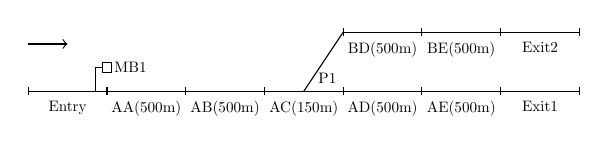
\begin{tikzpicture}[scale=0.5,transform shape]
\fontfamily{Heletvica Narrow}{\fontsize{11}{11}\selectfont
\draw [->] (0,-0.8) to (1,-0.8);

\RWConnector{a0}{(0,-2)}
\RWConnector{a1}{(2,-2)}
\RWLinearUnitBelow{a0}{a1}{Entry}
\RWSignal{MB1}{(2,-2)}{MB1}
\RWConnector{a2}{(4,-2)}
\RWLinearUnitBelow{a1}{a2}{AA(500m)}
\RWConnector{a3}{(6,-2)}
\RWLinearUnitBelow{a2}{a3}{AB(500m)}

\RWPoint{p101}{a4}{a5}{p101}{(7,-2)}
\RWLabelPointAboveLeft{a5}{a5}{P1}
\RWLabelLinearUnitBelow{a4}{a5}{AC(150m)}

\RWConnector{b6}{(10,-0.5)}
\RWLinearUnitBelow{p101}{b6}{BD(500m)}
\RWConnector{b7}{(12,-0.5)}
\RWLinearUnitBelow{b6}{b7}{BE(500m)}

\RWConnector{a6}{(10,-2)}
\RWLinearUnitBelow{a5}{a6}{AD(500m)}
\RWConnector{a7}{(12,-2)}
\RWLinearUnitBelow{a6}{a7}{AE(500m)}

\RWConnector{a8}{(14,-2)}
\RWLinearUnitBelow{a7}{a8}{Exit1}
\RWConnector{b8}{(14,-0.5)}
\RWLinearUnitBelow{b7}{b8}{Exit2}
}


\end{tikzpicture}
\quad \\
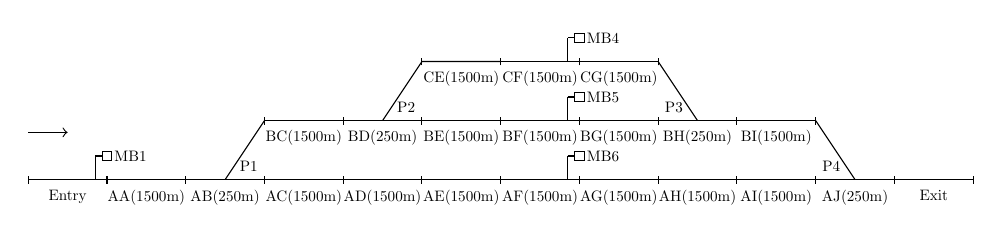
\begin{tikzpicture}[scale=0.5,transform shape]
\fontfamily{Heletvica Narrow}{\fontsize{11}{11}\selectfont
\draw [->] (0,-0.8) to (1,-0.8);

\RWConnector{a0}{(0,-2)}
\RWConnector{a1}{(2,-2)}
\RWLinearUnitBelow{a0}{a1}{Entry}
\RWSignal{MB1}{(2,-2)}{MB1}
\RWConnector{a2}{(4,-2)}
\RWLinearUnitBelow{a1}{a2}{AA(1500m)}
\RWPoint{p101}{a3}{a4}{p101}{(5,-2)}
\RWLabelPointAboveLeft{a4}{a4}{P1}
\RWLabelLinearUnitBelow{a3}{a4}{AB(250m)}

\RWConnector{b5}{(8,-0.5)}
\RWLinearUnitBelow{p101}{b5}{BC(1500m)}

\RWPoint{p102}{b6}{b7}{p102}{(9,-0.5)}
\RWLabelPointAboveLeft{b7}{b7}{P2}
\RWLabelLinearUnitBelow{b6}{b7}{BD(250m)}

\RWConnector{b8}{(12,-0.5)}
\RWLinearUnitBelow{b7}{b8}{BE(1500m)}
%\RWSignal{MB2}{(9,-0.5)}{MB2}

\RWConnector{a5}{(8,-2)}
\RWLinearUnitBelow{a4}{a5}{AC(1500m)}
%\RWSignal{MB3}{(9,-2)}{MB3}
\RWConnector{a6}{(10,-2)}
\RWLinearUnitBelow{a5}{a6}{AD(1500m)}


\RWConnector{c7}{(12,1)}
\RWLinearUnitBelow{p102}{c7}{CE(1500m)}
\RWConnector{c8}{(14,1)}
\RWLinearUnitBelow{c7}{c8}{CF(1500m)}
\RWSignal{MB2}{(14,1)}{MB4}
\RWConnector{c9}{(16,1)}
\RWLinearUnitBelow{c8}{c9}{CG(1500m)}

\RWConnector{b9}{(14,-0.5)}
\RWLinearUnitBelow{b8}{b9}{BF(1500m)}
\RWConnector{b10}{(16,-0.5)}
\RWLinearUnitBelow{b9}{b10}{BG(1500m)}
\RWSignal{MB3}{(14,-0.5)}{MB5}

\RWConnector{a7}{(12,-2)}
\RWLinearUnitBelow{a6}{a7}{AE(1500m)}
\RWConnector{a8}{(14,-2)}
\RWLinearUnitBelow{a7}{a8}{AF(1500m)}
\RWConnector{a9}{(16,-2)}
\RWLinearUnitBelow{a8}{a9}{AG(1500m)}
\RWSignal{MB4}{(14,-2)}{MB6}
\RWConnector{a10}{(18,-2)}
\RWLinearUnitBelow{a9}{a10}{AH(1500m)}
\RWConnector{a11}{(20,-2)}
\RWLinearUnitBelow{a10}{a11}{AI(1500m)}

\RWPointReverse{p103}{b11}{b12}{p103}{(17,-0.5)}
\RWLabelPointAboveRight{b12}{b12}{P3}
\RWLabelLinearUnitBelow{b11}{b12}{BH(250m)}

\RWConnector{b13}{(20,-0.5)}
\RWLinearUnitBelow{b11}{b13}{BI(1500m)}

\RWPointReverse{p104}{a12}{a13}{p104}{(21,-2)}
\RWLabelPointAboveRight{a13}{a13}{P4}
\RWLabelLinearUnitBelow{a12}{a13}{AJ(250m)}

\RWConnector{a14}{(24,-2)}
\RWLinearUnitBelow{a12}{a14}{Exit}
}
\end{tikzpicture}
\caption{Track plans for a junction and three platform station.}
\label{fig:junction}
\label{fig:threestation}
\end{figure}

We check all three track plans with manually constructed tables that
we consider to be correct. In all settings the model checking confirms
that these rail yard designs are collision free (within the given
time-bound, if applicable).  The table shows verification
times\footnote{Using a PC running Xubuntu
  14.04.2 with an i7 4790 @3.60Ghz and 32GB RAM.} and the number of
rewrite steps for the three rail yards against the random controller
and the round-robin controller (see Section~\ref{ssec:instan}).  The
following table presents our model checking results.
%
%% Here, we follow the finitisation technique given by James et
%% al.~\cite{sttt14}, namely that proving collision-freedom for two
%% trains is enough for proving safety in general. However, this result
%% requires a proof on based around the encoding of our railway DSL in
%% real-time maude.  Even though our encoding follows James at al's, this
%% proof remains as future work.
%

\vspace{-0.3cm}
\begin{table}
\centering
\caption{Verification results of model checking three scheme plans.}
{\small
  \begin{tabular}{|l|c|c|}
    \hline 
    \textbf{Scheme Plan} & \textbf{Round Robin Controller} &
    \textbf{Random Controller} \\
    & \textbf{Unbounded} & \textbf{in Time 300} \\
    \hline \hline
    Junction  & 0.5s / 1,465,601 rewrites & \hphantom{1}361.1s /   \hphantom{1}\hphantom{1}151,564,627 rewrites \\
    Pass-through Station & 0.7s  / 1,886,303  rewrites & \hphantom{1}589.0s /  \hphantom{1}\hphantom{1}500,397,040 rewrites \\
    Three Platform Station & 1.2s / 2,622,022  rewrites & 1957.9s / 1,009,144,410  rewrites \\
    \hline
 \end{tabular}
}
\end{table}
\vspace{-0.3cm}

%% \label{tab:results}
%% \end{figure}
%

The table shows that unbounded model checking is successful when
control is restricted, e.g., to our round-robin controller. This is due to the restrictions that such a control strategy puts on train movements through the sheme plan. However,
when using our random controller, the state space vastly
increases. Thus, we provide results for up to a given time bound of
$300s$. Note that this time is enough to ensure that two trains can
travel completely through the Junction and Station scheme
plan. As expected, model checking times increase with the complexity of the scheme plans. 
It is future work, to consider further, more varied rail
yards.

%%% Phil

\section{Related Work}
%%% Todo: Markus
ERTMS is a complex systems of systems, made up of distributed
components interconnected through standard (e.g.\ Euroradio) and
proprietary (e.g.\ Siemens-specific) protocols and algorithms. Our
approach reflects this by covering the full control cycle between
controller, interlocking, radio-block centre and trains. Our objective
is to verify the location specific data of railway designs in their
early development stages, accompanying a standard design process
performed by signalling companies such as our industrial partner
Siemens.

%% This is in
%% contrast to a number of other works, which focus on parts of ERTMS
%% only. 

%% Another
%% dimension is the question if the verification takes place on design or
%% implementation level.

Our approach to cover all components is different from several
verification approaches with a focus on a single component only.
%
Vu et al.~\cite{vu15} provide a generic and re-configurable model
of ERTMS Level 2 on the design level with the same objective that we
have. They present their model as a Kripke structure and verify
high-level safety properties such as head-to-head collision or
derailment on a point. %% They introduce a concept of virtual signals and
%% argue that this allows them to handle the assignment of movement
%% authorities in a way similar to the situation where conventional
%% signals are used. Their verification technology is SMT solving as
%% implemented in the RT-Tester tool-box. It is able to handle large
%% Danish rail stations.
Their approach
%
%% This reduction
abstracts from trains and the RBC and presumes these components to be
correctly implemented. Thus, their verification focuses on the
interlocking component.
%
%% %
%% On the modelling side, differences appear to be mostly due to national
%% pecularities. They model the Danish interlocking system, which is
%% based upon ``interlocking tables'' similar to our control
%% tables. Furthermore, they apply the technique of sequential
%% release. As we deal with uni-directional railways only, in our setting
%% release tables for points are sufficient.
%
Cimatti et al.~\cite{cimatti12} apply software model checking to
verify the implementation level a subsystem responsible for the
allocation of logical routes to trains. The software under
consideration has been developed by Ansaldo-STS and is part of this
company's implementation of ERTMS Level 2. %% An example of a property
%% under consideration is ``no two different trains occupy the same
%% track''.  Cimatti et al.\ represent the software in the VELOS
%% specification language (resembling the C++ language), the properties
%% of interest in temporal logic, and discuss in detail the performance
%% of different model checkers. Thus,
They focus on software verification of a sub-component rather than on
location specific data for the whole system.
%
Nardone et al.~\cite{nardone14} develop a new, rail specific
specification language DSTM4Rail, an extension of hierarchical state
machines. They employ DSTM4Rail to the modelling of specific
functionalities of the ERTMS Radio Block Centre. Overall the objective
is to obtain a formal model of ERTMS requirements for system testing
purposes. %% The long term goal is integration into a model-driven
%% development processes.
This work is specialised to quality assurance for one ERTMS component.

The openETCS initiative~\cite{openETCS} sets out to provide
specifications that can be used for software generation for ETCS train
control components, track elements, and functionality to be integrated
in track side interlocking systems. This software development follows
a model-driven approach, where the methods and tools shall comply with
a SIL 4 development process. 

Chiappini et al.~\cite{chiappini10} work towards the
formalisation and validation of the overall ERTMS/ETCS
specifications. To this end, they formalise a reference subset
(including Movement Authority Management and RBC/RBC Handover) of the
system requirements through a set of concepts and diagrams in UML, and
through additional constraints in a defined controlled natural
language. This formalisation then undergoes an automatic validation
check covering questions concerning consistency, scenario
compatibility, and if certain properties hold. Their work puts the
ERTMS/ETCS specifications themselves under scrutiny. Their methods are
semi-formal.





%%% Todo: Markus

\section{Summary and Future Work}

In this paper, we have modelled, validated, and verified a complex
system of systems of hybrid nature.
%
%
%
To this end, 
%
we presented an analysis of the ERTMS system,
%
described its information flow,
%
and provided a concise model in Real Time Maude. 
%
This model is astonishingly small: it consists of around only 1000
lines of code. We believe this is due to the advanced concepts,
especially the object orientated features that Real Time Maude offers.
%
Through simulation we have demonstrated that our model exhibits a
number of expected behaviours.
%
Furthermore, by systematic error injection, we have shown that safety
in ERTMS depends on all its components. 
%
This simulation and error injection give us confidence that our model
is valid.
%
Finally, we have presented a number of model checking results that
indicate that, for small rail yards, complexity of model checking of
time-dependent safety properties is under control.

It is future work to explore further, more complex rail yards,
including bi-directional ones. On the practical side we intend to
extend our modelling with further controller strategies and more
complex train progression behaviour. On the more theoretical side, we
plan to investigate completeness and abstraction techniques to reduce
model-checking time, including finitisation.

%%% Todo: Markus

\paragraph{Acknowledgement} 
The authors would like to thank Simon Chadwick, Siemens Rail
Automation, UK, for his continued support and many helpful
discussions. We also appreciate the helpful advice from  Peter \"Olveczky
%towards our modelling 
on Real-Time Maude and the constructive comments given by three anonymous referees. Finally, we thank Erwin R.\ Catesbeiana (Jr) for timely hints on how to
stay on track.

\bibliographystyle{abbrv}
\bibliography{doc}

\end{document}

